% Options for packages loaded elsewhere
\PassOptionsToPackage{unicode}{hyperref}
\PassOptionsToPackage{hyphens}{url}
%
\documentclass[
]{article}
\usepackage{amsmath,amssymb}
\usepackage{iftex}
\ifPDFTeX
  \usepackage[T1]{fontenc}
  \usepackage[utf8]{inputenc}
  \usepackage{textcomp} % provide euro and other symbols
\else % if luatex or xetex
  \usepackage{unicode-math} % this also loads fontspec
  \defaultfontfeatures{Scale=MatchLowercase}
  \defaultfontfeatures[\rmfamily]{Ligatures=TeX,Scale=1}
\fi
\usepackage{lmodern}
\ifPDFTeX\else
  % xetex/luatex font selection
\fi
% Use upquote if available, for straight quotes in verbatim environments
\IfFileExists{upquote.sty}{\usepackage{upquote}}{}
\IfFileExists{microtype.sty}{% use microtype if available
  \usepackage[]{microtype}
  \UseMicrotypeSet[protrusion]{basicmath} % disable protrusion for tt fonts
}{}
\makeatletter
\@ifundefined{KOMAClassName}{% if non-KOMA class
  \IfFileExists{parskip.sty}{%
    \usepackage{parskip}
  }{% else
    \setlength{\parindent}{0pt}
    \setlength{\parskip}{6pt plus 2pt minus 1pt}}
}{% if KOMA class
  \KOMAoptions{parskip=half}}
\makeatother
\usepackage{xcolor}
\usepackage[margin=1in]{geometry}
\usepackage{graphicx}
\makeatletter
\def\maxwidth{\ifdim\Gin@nat@width>\linewidth\linewidth\else\Gin@nat@width\fi}
\def\maxheight{\ifdim\Gin@nat@height>\textheight\textheight\else\Gin@nat@height\fi}
\makeatother
% Scale images if necessary, so that they will not overflow the page
% margins by default, and it is still possible to overwrite the defaults
% using explicit options in \includegraphics[width, height, ...]{}
\setkeys{Gin}{width=\maxwidth,height=\maxheight,keepaspectratio}
% Set default figure placement to htbp
\makeatletter
\def\fps@figure{htbp}
\makeatother
\setlength{\emergencystretch}{3em} % prevent overfull lines
\providecommand{\tightlist}{%
  \setlength{\itemsep}{0pt}\setlength{\parskip}{0pt}}
\setcounter{secnumdepth}{-\maxdimen} % remove section numbering
\ifLuaTeX
  \usepackage{selnolig}  % disable illegal ligatures
\fi
\IfFileExists{bookmark.sty}{\usepackage{bookmark}}{\usepackage{hyperref}}
\IfFileExists{xurl.sty}{\usepackage{xurl}}{} % add URL line breaks if available
\urlstyle{same}
\hypersetup{
  pdftitle={Area Analysis},
  pdfauthor={Jaxson Freund},
  hidelinks,
  pdfcreator={LaTeX via pandoc}}

\title{Area Analysis}
\author{Jaxson Freund}
\date{2024-02-27}

\begin{document}
\maketitle

\hypertarget{data}{%
\subsection{Data}\label{data}}

\begin{verbatim}
## # A tibble: 1,550 x 2
##    Distance  Area
##    <fct>    <dbl>
##  1 -2       0.781
##  2 -2       0.874
##  3 -2       1.45 
##  4 -2       0.443
##  5 -2       1.16 
##  6 -2       0.863
##  7 -2       0.81 
##  8 -2       1.05 
##  9 -2       1.03 
## 10 -2       0.939
## # i 1,540 more rows
\end{verbatim}

\hypertarget{visualize-the-data}{%
\subsection{Visualize the data}\label{visualize-the-data}}

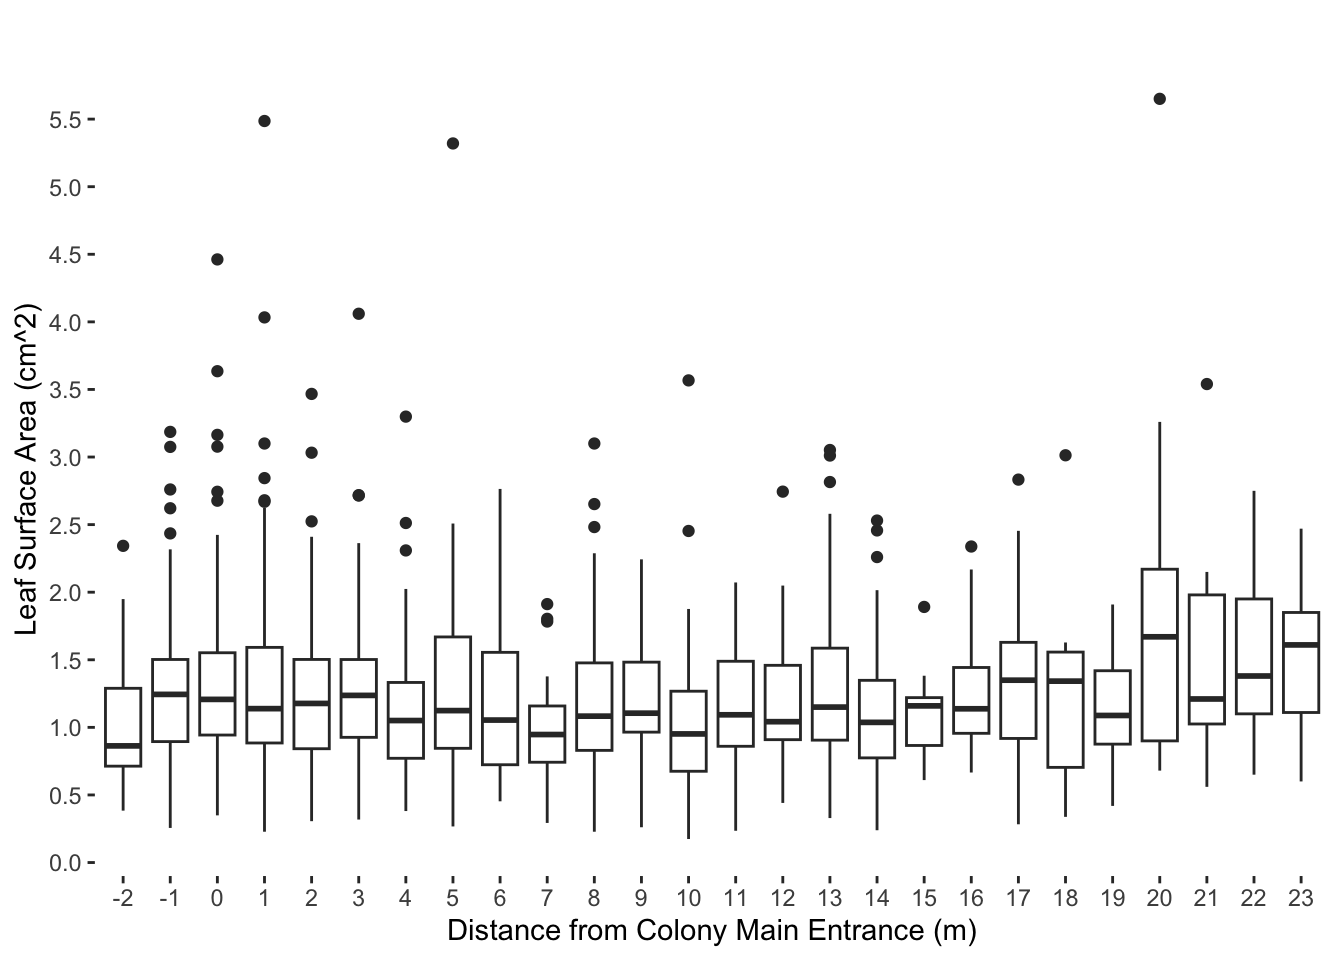
\includegraphics{area_analysis_files/figure-latex/unnamed-chunk-3-1.pdf}
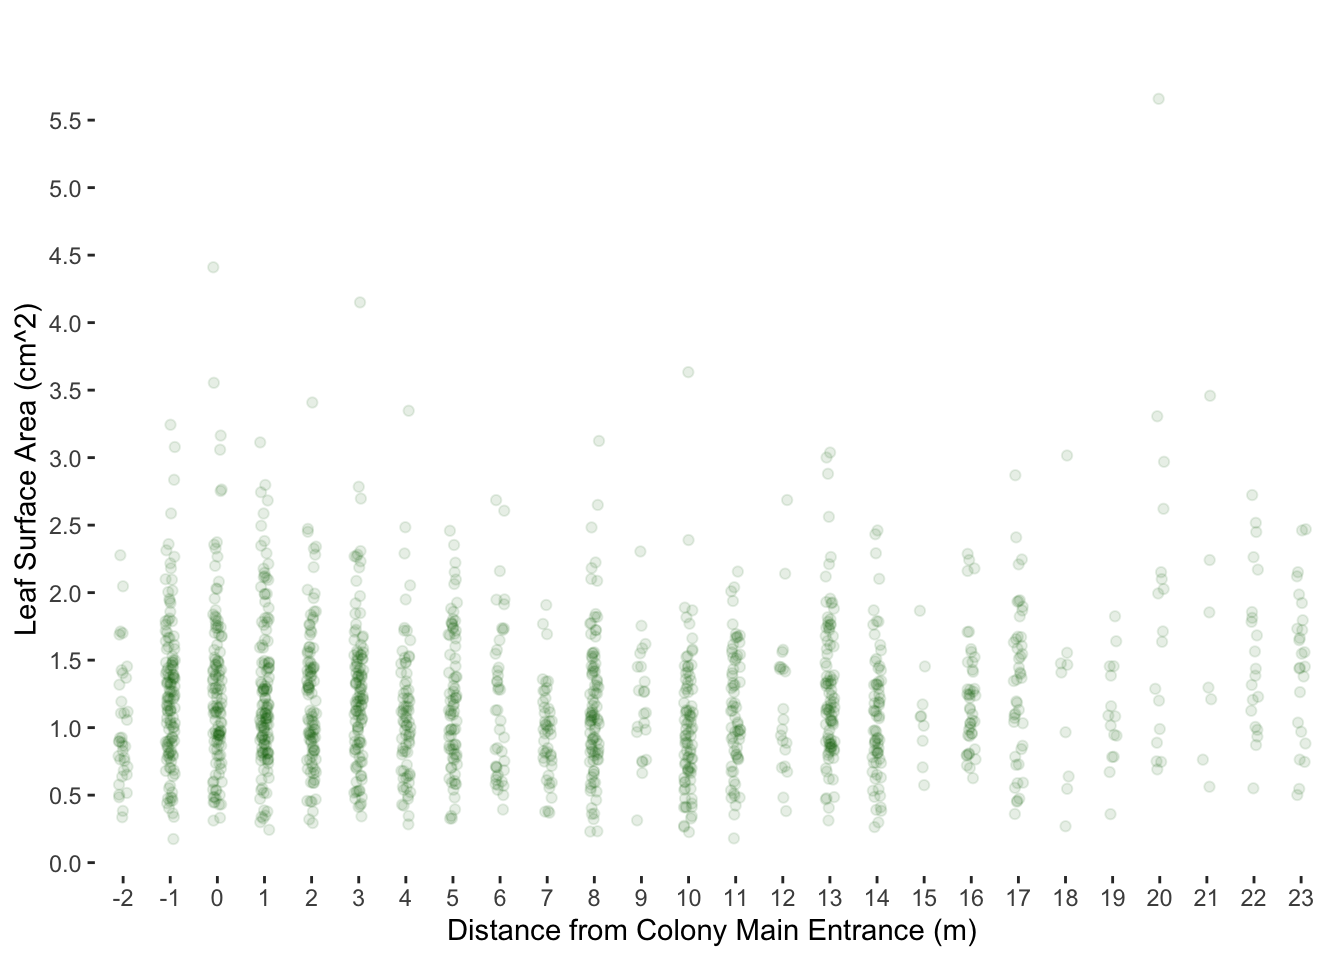
\includegraphics{area_analysis_files/figure-latex/unnamed-chunk-3-2.pdf}
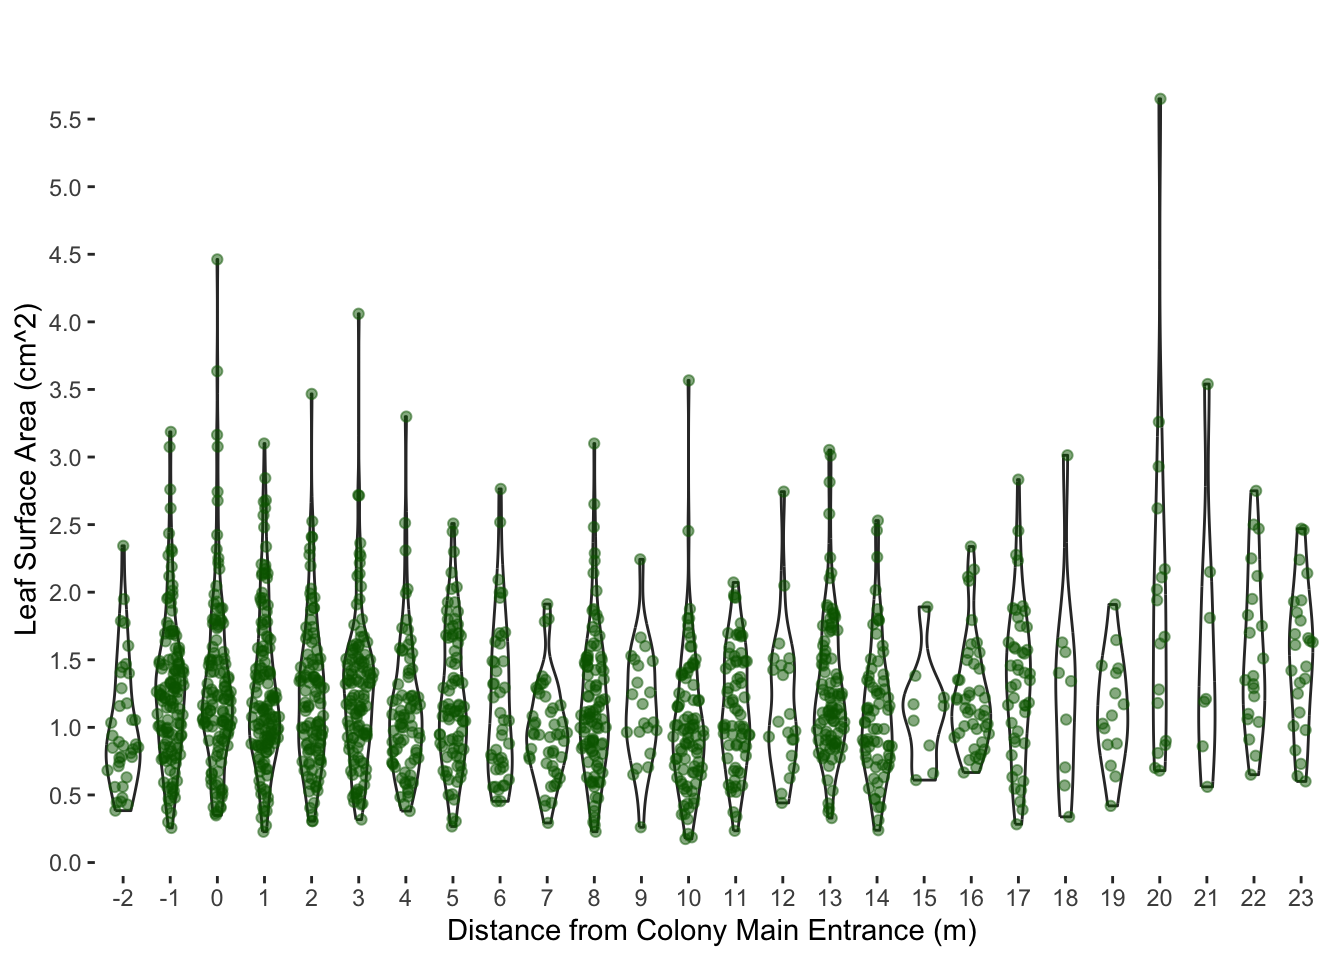
\includegraphics{area_analysis_files/figure-latex/unnamed-chunk-3-3.pdf}
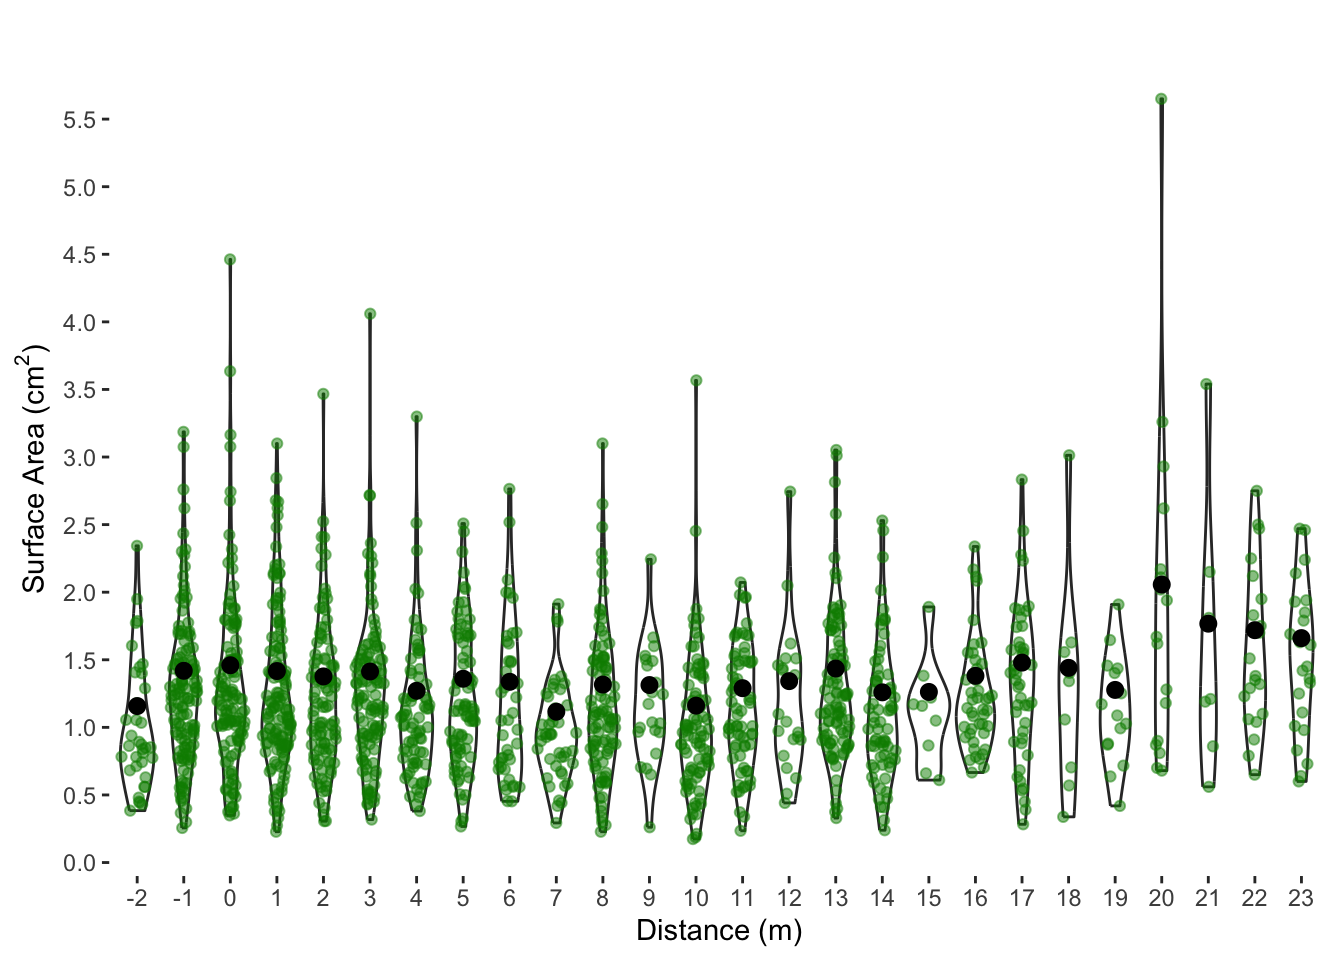
\includegraphics{area_analysis_files/figure-latex/unnamed-chunk-3-4.pdf}

\begin{verbatim}
## # A tibble: 26 x 3
##    Distance  Mean     SE
##    <fct>    <dbl>  <dbl>
##  1 -2       1.01  0.0767
##  2 -1       1.27  0.0474
##  3 0        1.31  0.0590
##  4 1        1.27  0.0499
##  5 2        1.23  0.0527
##  6 3        1.26  0.0511
##  7 4        1.12  0.0577
##  8 5        1.21  0.0568
##  9 6        1.19  0.0876
## 10 7        0.966 0.0524
## # i 16 more rows
\end{verbatim}

\hypertarget{statistics}{%
\subsection{Statistics}\label{statistics}}

\begin{verbatim}
##               Df Sum Sq Mean Sq F value   Pr(>F)    
## Distance      25   27.8  1.1121   3.685 2.74e-09 ***
## Residuals   1524  459.9  0.3018                     
## ---
## Signif. codes:  0 '***' 0.001 '**' 0.01 '*' 0.05 '.' 0.1 ' ' 1
\end{verbatim}

\begin{verbatim}
## $statistics
##     MSerror   Df     Mean       CV
##   0.3017987 1524 1.220206 45.02206
## 
## $parameters
##    test   name.t ntr StudentizedRange alpha
##   Tukey Distance  26         5.210735  0.05
## 
## $means
##         Area       std   r         se   Min   Max     Q25    Q50     Q75
## -1 1.2685682 0.5440600 132 0.04781583 0.256 3.186 0.89475 1.2440 1.50225
## -2 1.0075946 0.4666685  37 0.09031457 0.384 2.343 0.71300 0.8630 1.28900
## 0  1.3095806 0.6564874 124 0.04933417 0.349 4.462 0.94325 1.2070 1.55200
## 1  1.2668134 0.5776422 134 0.04745765 0.228 3.100 0.88350 1.1340 1.58075
## 10 1.0106136 0.5150416  88 0.05856219 0.174 3.567 0.67525 0.9515 1.26750
## 11 1.1398406 0.4386382  69 0.06613542 0.235 2.072 0.86000 1.0930 1.48900
## 12 1.1920952 0.5417438  21 0.11988063 0.441 2.744 0.90900 1.0420 1.45900
## 13 1.2853053 0.5317337  95 0.05636336 0.329 3.052 0.90550 1.1500 1.58600
## 14 1.1091429 0.4891396  70 0.06566133 0.239 2.530 0.77425 1.0370 1.34800
## 15 1.1121111 0.3901543   9 0.18312069 0.610 1.891 0.86600 1.1590 1.22000
## 16 1.2313409 0.4054133  44 0.08281945 0.666 2.338 0.95600 1.1375 1.44300
## 17 1.3291778 0.5662934  45 0.08189406 0.283 2.833 0.91800 1.3490 1.62900
## 18 1.2903333 0.7899096   9 0.18312069 0.338 3.013 0.70400 1.3420 1.55700
## 19 1.1270667 0.4003059  15 0.14184468 0.419 1.909 0.87600 1.0880 1.41900
## 2  1.2268774 0.5430265 106 0.05335876 0.306 3.467 0.84100 1.1690 1.49575
## 20 1.9064706 1.2458729  17 0.13323987 0.680 5.650 0.90000 1.6700 2.17000
## 21 1.6171429 1.0047838   7 0.20763935 0.560 3.540 1.02500 1.2100 1.98000
## 22 1.5690476 0.5954150  21 0.11988063 0.650 2.750 1.10000 1.3800 1.95000
## 23 1.5104000 0.5356575  25 0.10987241 0.600 2.470 1.11000 1.6100 1.85000
## 3  1.2631379 0.5508285 116 0.05100699 0.318 4.060 0.92625 1.2365 1.50200
## 4  1.1206974 0.5026705  76 0.06301615 0.381 3.299 0.77125 1.0505 1.33225
## 5  1.2098148 0.5112562  81 0.06104023 0.267 2.508 0.84400 1.1210 1.66300
## 6  1.1871860 0.5744438  43 0.08377693 0.453 2.764 0.72350 1.0540 1.55500
## 7  0.9659348 0.3553319  46 0.08099902 0.293 1.912 0.74200 0.9470 1.15825
## 8  1.1664694 0.5291474  98 0.05549395 0.228 3.100 0.82975 1.0830 1.47700
## 9  1.1631364 0.4310594  22 0.11712439 0.261 2.243 0.96475 1.1050 1.48250
## 
## $comparison
## NULL
## 
## $groups
##         Area groups
## 20 1.9064706      a
## 21 1.6171429     ab
## 22 1.5690476     ab
## 23 1.5104000     ab
## 17 1.3291778      b
## 0  1.3095806      b
## 18 1.2903333      b
## 13 1.2853053      b
## -1 1.2685682      b
## 1  1.2668134      b
## 3  1.2631379      b
## 16 1.2313409      b
## 2  1.2268774      b
## 5  1.2098148      b
## 12 1.1920952      b
## 6  1.1871860      b
## 8  1.1664694      b
## 9  1.1631364      b
## 11 1.1398406      b
## 19 1.1270667      b
## 4  1.1206974      b
## 15 1.1121111      b
## 14 1.1091429      b
## 10 1.0106136      b
## -2 1.0075946      b
## 7  0.9659348      b
## 
## attr(,"class")
## [1] "group"
\end{verbatim}

\end{document}
